\documentclass[conference]{IEEEtran}
\IEEEoverridecommandlockouts
% The preceding line is only needed to identify funding in the first footnote. If that is unneeded, please comment it out.
\usepackage{cite}
\usepackage{amsmath,amssymb,amsfonts}
\usepackage{algorithmic}
\usepackage{graphicx}
\usepackage{textcomp}
\usepackage{xcolor}
\def\BibTeX{{\rm B\kern-.05em{\sc i\kern-.025em b}\kern-.08em
    T\kern-.1667em\lower.7ex\hbox{E}\kern-.125emX}}
\begin{document}

\title{Performance Comparison of Several Neural Networks in Policy
Approximation in a Ludo Game Playing Agent}

\author{

\IEEEauthorblockN{Kartik Tushir}
\IEEEauthorblockA{
kk1478@msstate.edu
}

\and

\IEEEauthorblockN{Rajeev Jogi}
\IEEEauthorblockA{
rj993@msstate.edu
}

\and

\IEEEauthorblockN{James Kastrantas}
\IEEEauthorblockA{
jgk16@msstate.edu
}

}

\maketitle

\begin{IEEEkeywords}
  reinforcement learning, policy approximation, ludo, deep learning, gradient
  ascent, experience replay
\end{IEEEkeywords}

\section{Task Definition}

Our task for this project is to determine which neural network models work
best for a reinforcement learning agent playing the game of Ludo. A recurrent
neural network (RNN), convolutional neural network (CNN), and fully-connected
artifical neural network (ANN) will be used to approximate a policy for the
game.

\begin{figure}[htbp]
    \centerline{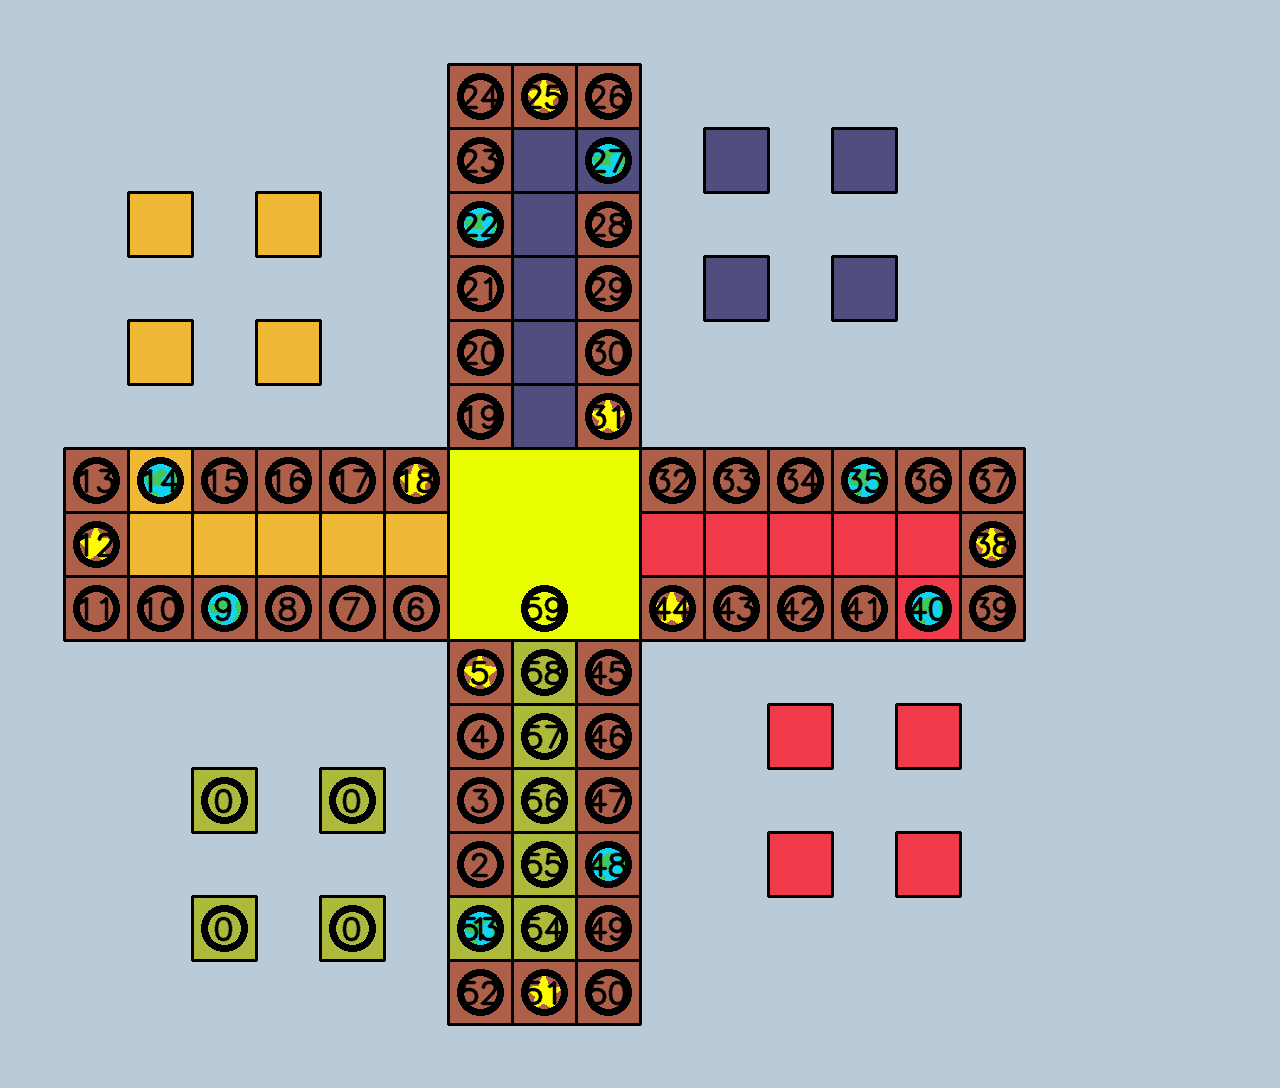
\includegraphics[width=7cm, height=7cm]{fig1.png}}
    \caption{A Ludo game board labeled with encodings for pawn positions. [1]}
    \label{fig}
\end{figure}

Ludo is a game in which each player tries to move their four pawns from the
starting position to the goal in the center of the board. Player can move one
of their pawns from one to six spaces decided by a six-sided die roll. A
player can remove another player's pawn by moving into the opposing pawn's
space, but there are areas of the board where opposing players cannot be
reached or are immune to removal. The action available to a player is the
decision of which pawn to move. This decision must be weighed against the
current state of the game, making some pawns better to move than others. The
agents must be trained to learn these strategies.

\section{Literature Review}

\subsection{Reinforcement Learning: An Introduction [2]}

A more in-depth discussion of policy approximation is given in the section on
policy gradient methods. Advantages of policy approximation are given, but
missing are discussions on the disadvantages to policy approximation.
Converging on a policy approximation by computing the Monte-Carlo policy
gradient will be essential for estimating a policy, and that is outlined here.

\subsection{Reinforcement Learning for Robots Using Neural Networks [3]}

A dissertation that provides techniques for effective reinforcement learning.
The background provides an excellent introduction to reinforcement learning.
Discussed is hierarchical learning, using smaller elementary problems that can
agent can solve which can be used to learn strategies for more complex
problems. Experience from human teachers to improve training is discussed.
Experience replay, which is essential for assigning rewards to state-action
pairs, is also discussed. All of these topics may be useful to training our
agents.

\subsection{Q-Learning [4]}

This technichal note proves that Q-learning converges on an optimal policy.
It serves as a short introduction on Q-learning, and elaborates on the
relationship between Q-learning and dynamic programming. It also shows that
each problem instance may have multiple optimal policies, but each
state-action pair $(s, a)$ has a unique Q-value $Q(s, a)$. Using the
state-action pair that maximizes the Q-value is the same as having an optimal
policy $\pi^*$. This is important because the reward table $\mathcal{R}$ and
transition probability table $P_{xy}$ may not be known ahead of time, or is
too large to compute beforehand, and using Q-learning eliminates the need for
these resource-intensive models.

\section{Motivation}

It is in our experience that teaching concepts to others is the best way to
learn those concepts. The motivation for the project comes from the
requirements for the class, but the final result will be shaped as an
assignment appropriate for an introductory, undergraduate level AI class,
complete with implementation for them to get started with.

In a two-player game of Ludo, there are no more than 2 quadrillion possible
states of the game. While not impossible, utilizing immense amounts of
secondary memory is necessary to compute a policy table. A reinforcement
learning agent that can generalize from experience and approximate this table
using a neural network would be beneficial for both people training the agent
and people running the agent on limited computational resources such as
personal computers or smartphones. 

Simply explaining to students how these agents work does not provide a good
hands-on experience for students learning reinforcement learning. Forming an
assignment that gives them a completely-observable, zero-sum game with a large
state space that makes it very, very difficult to compute and store a policy
table for the game, we can give them the experience they need to design their
own reinforcement learning agents. This can lead into discussion on larger
problems complicated by partial-observability.

\section{Methods}

Adapting LUDOpy from the GitHub repository as the implementation of the
environment, we are going to train several reinforcement learning agents to
learn and compete at a 2-player game of Ludo.  Although Ludo can be played
with 4 players, 2 players will be used in training the agents to simplify
the state space.

Episodes generated by LUDOpy's random walks will allow the agents to assign
rewards to states based on their future outcomes. Gradient ascent will be used
to adjust the weights of the policy network since this is a maximization
problem.

Several neural network models for policy approximation: RNN, CNN, and
fully-connected ANN. This will allow students working in groups to distribute
training tasks evenly, and allow them to compare game-playing performance of
their agents.

\section{Evaluation}

We will see which networks best maximize future rewards by measuring future
rewards from the initial state. We can also setup brackets and play games
against the other agents and determine which agent wins more games. Parameter
size is also a factor we will consider. We can also look at adjustments to the
hyperparameters of the network to see which models converge faster according
to a different learning rate or depth of the network.

\begin{thebibliography}{00}
\bibitem{b1} SimonLBSoerensen, LUDOpy, GitHub repository,
    https://github.com/SimonLBSoerensen/LUDOpy, 2020.
\bibitem{b2} R. S. Sutton and A. G. Barto, Reinforcement Learning: An
    Introduction, 2nd ed. Cambridge: MIT Press, 2020. Accessed on Sep. 26,
        2020. [Online]. Available:
        http://incompleteideas.net/sutton/book/RLbook2020.pdf
\bibitem{b3} Long-Ji Lin, "Reinforcement learning for robots using neural
    networks," Ph. D dissertation, School of Computer Science, Carnegie Mellon
        Univ., Pittsburgh, 1993. Accessed on Sep. 11, 2020. [Online].
        Available: http://isl.anthropomatik.kit.edu/pdf/Lin1993.pdf
\bibitem{b4} C. J. C. H. Watkins, P. Dayan, "Q-Learning," Machine Learning,
    vol. 8, pp. 279-292, May 1992.
\end{thebibliography}
\vspace{12pt}

\end{document}

